\chapter{Resoconto delle attività di verifica}\label{resoconto}
\section{Analisi}\label{Analisi}
Nel periodo antecedente la Revisione dei Requisiti sono stati verificati i documenti ed i processi applicando quanto descritto nelle \textit{Norme di Progetto v2.0.0}.\\
L'analisi statica è stata effettuata secondo i criteri e le modalità indicate nelle \textit{Norme di Progetto}.\\ 
Per gli errori riscontrati effettuando \textit{walkthrough$_{G}$}, si è provveduto a correggere le anomalie riscontrate e sono stati riportati nella lista di controllo nelle \textit{Norme di Progetto v2.0.0} per permettere di effettuare inspection successivamente.\\
L'\textit{inspection$_{G}$} viene effettuata utilizzando la lista di controllo precedentemente stilata. \\
Si sono poi calcolate le metriche descritte nelle \textit{Norme di Progetto}.\\
L'avanzamento dei processi viene poi valutato secondo le metriche descritte nelle \textit{Norme di Progetto}. 
\subsection{Verifica dei processi}
Per il\glossario{processo}di stesura dei documenti, il calcolo delle metriche di Budget Variance e di Schedule Variance è stato effettuato sul valore complessivo delle ore impiegate dal totale dei componenti del gruppo.\\
Per le successive fasi del \textit{progetto$_{G}$}, il gruppo si propone di automatizzare il processo di calcolo delle ore impiegate, con il dettaglio puntuale dei singoli processi.
Lo Schedule Variance totale è di -1 ore e il Budget Variance totale equivale a -25\euro.
\begin{comment}
\begin{tabularx}{\textwidth}{|C|C|C|}
	\hline
	\textbf{Macro-Attività}& \textbf{SV}&\textbf{BV}\\
	\hline
	\textit{Norme di Progetto}    & \euro & \euro\\
	\textit{Piano di Progetto}    & \euro & \euro\\
	\textit{Studio di Fattibilità} & \euro & \euro\\
	\textit{Analisi dei Requisiti}& \euro & \euro\\
	\textit{Piano di Qualifica}   & \euro & \euro\\
	\textit{Glossario}            & \euro & \euro\\
	\hline
	\caption{Esito verifica processi}
\end{tabularx}
\end{comment}
\\
\subsection{Verifica dei documenti}
\begin{tabularx}{\textwidth}{|C|c|C|}
	\hline
	\textbf{Documento}& \textbf{Indice di Gulpease}&\textbf{Esito}\\
	\hline
	\endhead
	\textit{Norme di Progetto}    & 76 & Superato \\
	\textit{Piano di Progetto}    & 64 & Superato \\
	\textit{Studio di Fattibilità} & 61 & Superato\\
	\textit{Analisi dei Requisiti}& 80 & Superato \\
	\textit{Piano di Qualifica}   & 67 & Superato \\
	\textit{Glossario}            & 68 & Superato \\
	\hline
	\caption{Esito della verifica documenti}
\end{tabularx}

\section{Revisione Analisi}
\label{revisione}
Durante il breve periodo di Revisione Analisi, il gruppo si è preparato allo sviluppo del POC e ha apportato delle correzione ai documenti, migliorando i propri processi. 
\subsection{Verifica dei processi}
I miglioramenti principali (tutti descritti nelle \textit{Norme di Progetto v2.0.0}) sono stati:
\begin{itemize}
	\item Automatizzato il calcolo delle ore di lavoro integrando\glossario{Harvest}ad \textit{Asana$_{G}$};
	\item Automatizzato il calcolo dell'\textit{Indice di Gulpease$_{G}$}, tramite script;
	\item Se dei documenti contenenti degli errori grammaticali raggiungono la repository, un bot avvisa per email chi ha commesso l'errore e invia una notifica al gruppo.
\end{itemize}

\subsubsection{MP001 Schedule variance}
Durante il periodo di Revisione Analisi 
\begin{figure} [h]
    \centering
	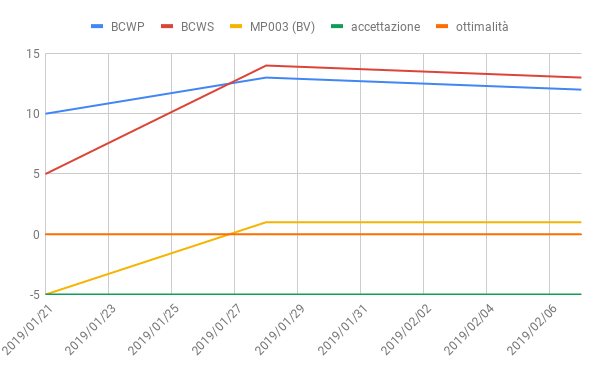
\includegraphics[scale=0.5]{./images/svRa.png}
	\caption{\textit{MP001 - Revisione Analisi}}\label{}
\end{figure}
\pagebreak
\subsubsection{MP002 Budget variance}
\begin{figure} [h]
    \centering
	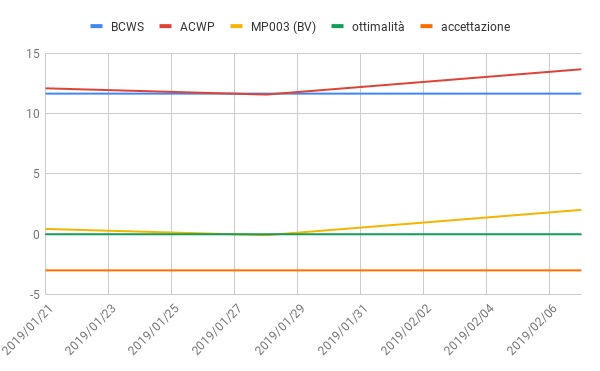
\includegraphics[scale=0.5]{./images/bvra.png}
	\caption{\textit{MP002 - Revisione Analisi}}\label{}
\end{figure}
\section{Progettazione della base tecnologica}
\label{progettazione}
\subsection{MP001: Schedule variance}
A causa di un imprevisto successo all'interno del gruppo con la tecnologia \textit{API}\glossario{Gateway}c'è stato un innalzamento dello schedule variance che ha raggiunto il picco ai primi di marzo.
\begin{figure} [h]
    \centering
	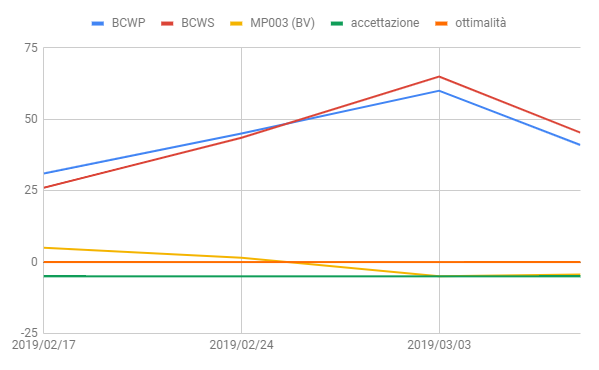
\includegraphics[scale=0.6]{./images/svP.png}
	\caption{\textit{MP001 - Progettazione della base tecnologica}}\label{}
\end{figure}
\pagebreak
\subsection{MP002: Budget variance}
\begin{figure} [h]
    \centering
	\includegraphics[scale=0.5]{./images/bvP.png}
	\caption{\textit{MP002 - Progettazione della base tecnologica}}\label{}
\end{figure}

\subsection{MP003: SPICE capability level}
Di seguito vengono riportati i livelli di maturità raggiunti dai processi eseguiti durante lo sviluppo del \textit{Proof of Concept$_{G}$}. Data l'inesperienza, non viene raggiunto il livello di accettazione richiesto (3) per la maggior parte dei processi, ma il gruppo sta lavorando per migliorare.
\begin{figure} [h]
    \centering
	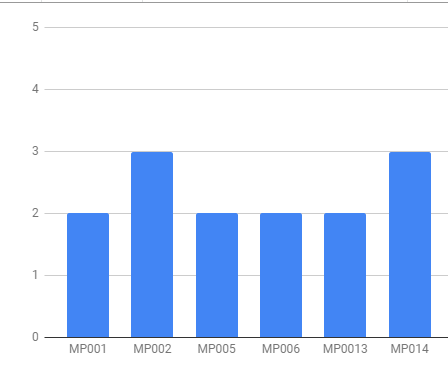
\includegraphics[scale=0.5]{./images/15504.png}
    \caption{\textit{MP003 - ISO/IEC 15504 }}\label{}
\end{figure}

\subsection{MP005:  Occorrenza rischi non previsti}
\textbf{Rischi non previsti: 2}
\begin{itemize}
	\item Un aggiornamento automatico di\glossario{Android Studio}ha completamente rimosso una libreria utilizzata dall'applicazione mobile, quindi il gruppo ha perso tempo per implementane una alternativa. Questo è successo perché la libreria in questione era deprecata. Per evitare problemi simili, l'utilizzo di librerie deprecate è stato vietato, come descritto nelle \textit{Norme di Progetto};
	\item É stata inserita una chiave di accesso Amazon nel repository. Il gruppo è stato avvisato da Amazon, e ha dovuto creare nuove chiavi per tutti i membri.
\end{itemize}

\subsection{MP006: Indisponibilità dei servizi}
\textbf{Indisponibilità dei servizi: 0}\\
Durante il periodo di progettazione della base tecnologica, il gruppo non ha riscontrato problemi riguardanti il downtime di servizi esterni.

\subsection{MP013: Percentuale build superate}
Viene fatta distinzione tra Android e Skill, in quanto vengono contenute in repository diversi.\\
Le build non superate sono 24 su 134 per la Skill e 29 su 232 per Android. Entrambe superano il range di ottimalità (80\%).
\begin{figure} [h]
    \centering
	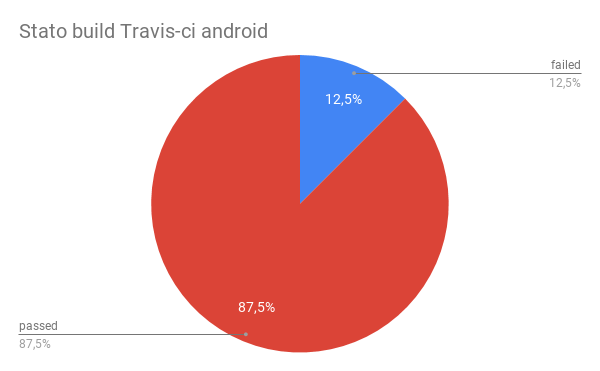
\includegraphics[scale=0.5]{./images/StatobuildTravis-ciandroid.png}
    \caption{\textit{MP013 - Android - Progettazione della base tecnologica}}\label{}
\end{figure}\\
\begin{figure} [h]
    \centering
	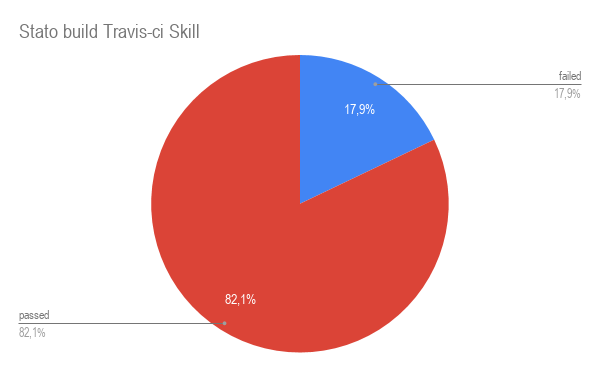
\includegraphics[scale=0.5]{./images/StatobuildTravis-ciSkill.png}
    \caption{\textit{MP013 - Skill - Progettazione della base tecnologica}}\label{}
\end{figure}
\clearpage

\subsection{MP014: Media commit giornaliera}
Come si può vedere dai grafici, il numero di commit è stato abbastanza costante, con un aumento del carico di lavoro durante la fine di febbraio.
\begin{figure} [h]
    \centering
	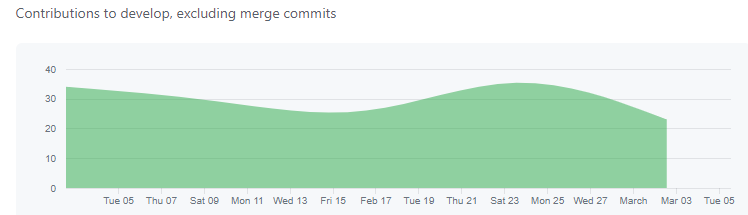
\includegraphics[scale=0.5]{./images/dailycommits_kotlin.PNG}
    \caption{\textit{MP014 - Android - Progettazione della base tecnologica}}
\end{figure}
\begin{figure} [h]
    \centering
	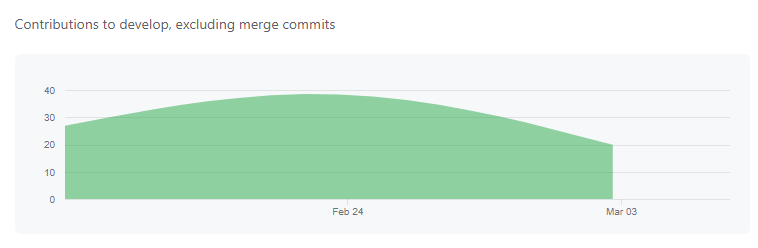
\includegraphics[scale=0.5]{./images/daycommits_js.PNG}
    \caption{\textit{MP014 - Skill - Progettazione della base tecnologica}}
\end{figure}

\subsection{MP015, MP016: Percentuale requisiti soddisfatti}
\begin{figure} [h]
    \centering
	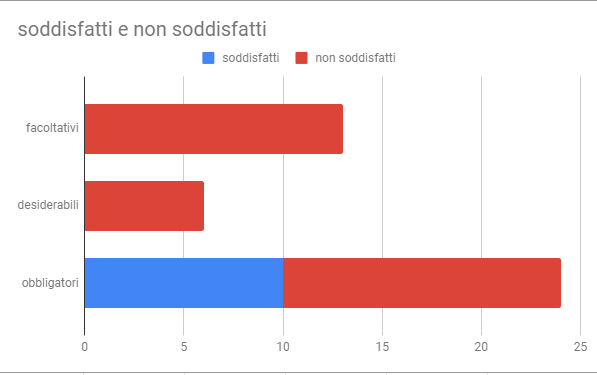
\includegraphics[scale=0.5]{./images/req.PNG}
    \caption{\textit{MP015 - MP016 Tipologia di requisiti}}
\end{figure}
\begin{figure} [h]
    \centering
	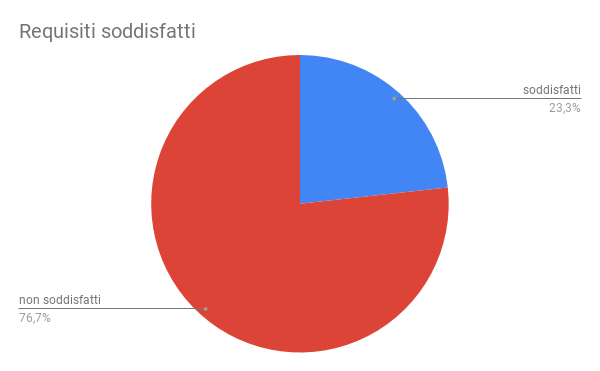
\includegraphics[scale=0.5]{./images/RequisitiSoddisfatti.png}
    \caption{\textit{MP015 - MP016 Differenza soddisfatti e non soddisfatti}}
\end{figure}
\subsection{MPR001 Ortografia}
Grazie allo script per la segnalazione automatica degli errori, questi vengono corretti a ogni push nel develop. Durante la verifica, comunque, sono stati trovati da zero a due errori per documento passati allo script. 
\subsection{MPR002 Indice di Gulpease}
\begin{figure} [h]
    \centering
	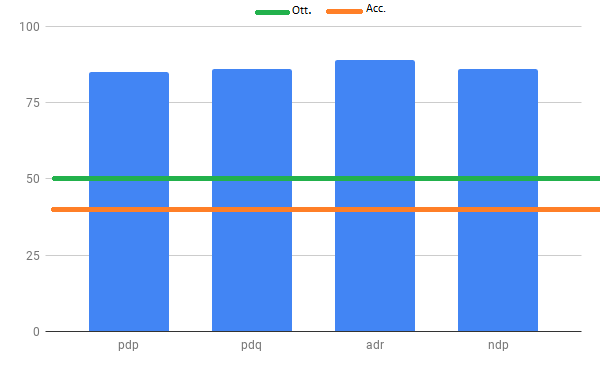
\includegraphics[scale=0.5]{./images/gulpeaseP.png}
    \caption{\textit{MPR002 \textit{Indice di Gulpease$_{G}$}}}
\end{figure}
\newpage
\section{Progettazione di dettaglio e codifica}
Questa sezione verrà compilata alla fine del periodo di Progettazione della base tecnologica.
\section{Verifica e collaudo}
Questa sezione verrà compilata alla fine del periodo di Verifica e collaudo.